% Created by tikzDevice version 0.12.3.1 on 2021-06-30 17:00:03
% !TEX encoding = UTF-8 Unicode
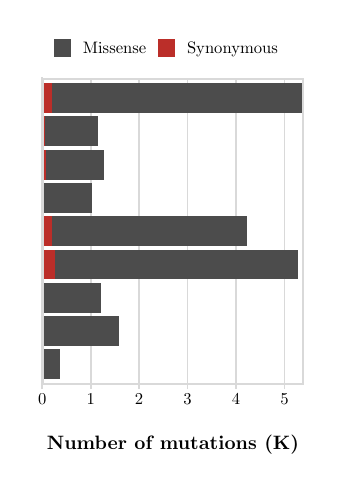
\begin{tikzpicture}[x=1pt,y=1pt]
\definecolor{fillColor}{RGB}{255,255,255}
\path[use as bounding box,fill=fillColor,fill opacity=0.00] (0,0) rectangle (103.28,157.19);
\begin{scope}
\path[clip] (  5.25, 28.30) rectangle ( 99.78,138.99);
\definecolor{drawColor}{gray}{0.85}

\path[draw=drawColor,line width= 0.6pt,line join=round] (  5.25, 28.30) --
	(  5.25,138.99);

\path[draw=drawColor,line width= 0.6pt,line join=round] ( 22.77, 28.30) --
	( 22.77,138.99);

\path[draw=drawColor,line width= 0.6pt,line join=round] ( 40.28, 28.30) --
	( 40.28,138.99);

\path[draw=drawColor,line width= 0.6pt,line join=round] ( 57.80, 28.30) --
	( 57.80,138.99);

\path[draw=drawColor,line width= 0.6pt,line join=round] ( 75.31, 28.30) --
	( 75.31,138.99);

\path[draw=drawColor,line width= 0.6pt,line join=round] ( 92.83, 28.30) --
	( 92.83,138.99);
\definecolor{fillColor}{gray}{0.30}

\path[fill=fillColor] (  8.74,126.36) rectangle ( 99.78,137.18);
\definecolor{fillColor}{RGB}{187,46,41}

\path[fill=fillColor] (  5.25,126.36) rectangle (  8.74,137.18);
\definecolor{fillColor}{gray}{0.30}

\path[fill=fillColor] (  6.25,114.33) rectangle ( 25.25,125.15);
\definecolor{fillColor}{RGB}{187,46,41}

\path[fill=fillColor] (  5.25,114.33) rectangle (  6.25,125.15);
\definecolor{fillColor}{gray}{0.30}

\path[fill=fillColor] (  6.56,102.29) rectangle ( 27.44,113.12);
\definecolor{fillColor}{RGB}{187,46,41}

\path[fill=fillColor] (  5.25,102.29) rectangle (  6.56,113.12);
\definecolor{fillColor}{gray}{0.30}

\path[fill=fillColor] (  5.25, 90.26) rectangle ( 23.22,101.09);

\path[fill=fillColor] (  8.93, 78.23) rectangle ( 79.36, 89.06);
\definecolor{fillColor}{RGB}{187,46,41}

\path[fill=fillColor] (  5.25, 78.23) rectangle (  8.93, 89.06);
\definecolor{fillColor}{gray}{0.30}

\path[fill=fillColor] (  9.87, 66.20) rectangle ( 97.73, 77.03);
\definecolor{fillColor}{RGB}{187,46,41}

\path[fill=fillColor] (  5.25, 66.20) rectangle (  9.87, 77.03);
\definecolor{fillColor}{gray}{0.30}

\path[fill=fillColor] (  5.81, 54.17) rectangle ( 26.62, 65.00);
\definecolor{fillColor}{RGB}{187,46,41}

\path[fill=fillColor] (  5.25, 54.17) rectangle (  5.81, 65.00);
\definecolor{fillColor}{gray}{0.30}

\path[fill=fillColor] (  5.25, 42.14) rectangle ( 32.87, 52.97);

\path[fill=fillColor] (  5.43, 30.11) rectangle ( 11.78, 40.94);
\definecolor{fillColor}{RGB}{187,46,41}

\path[fill=fillColor] (  5.25, 30.11) rectangle (  5.43, 40.94);

\path[draw=drawColor,line width= 1.1pt,line join=round,line cap=round] (  5.25, 28.30) rectangle ( 99.78,138.99);
\end{scope}
\begin{scope}
\path[clip] (  0.00,  0.00) rectangle (103.28,157.19);
\definecolor{drawColor}{gray}{0.85}

\path[draw=drawColor,line width= 0.6pt,line join=round,line cap=rect] (  5.25, 28.30) --
	(  5.25,138.99);
\end{scope}
\begin{scope}
\path[clip] (  0.00,  0.00) rectangle (103.28,157.19);
\definecolor{drawColor}{gray}{0.85}

\path[draw=drawColor,line width= 0.6pt,line join=round] (  5.25, 26.55) --
	(  5.25, 28.30);

\path[draw=drawColor,line width= 0.6pt,line join=round] ( 22.77, 26.55) --
	( 22.77, 28.30);

\path[draw=drawColor,line width= 0.6pt,line join=round] ( 40.28, 26.55) --
	( 40.28, 28.30);

\path[draw=drawColor,line width= 0.6pt,line join=round] ( 57.80, 26.55) --
	( 57.80, 28.30);

\path[draw=drawColor,line width= 0.6pt,line join=round] ( 75.31, 26.55) --
	( 75.31, 28.30);

\path[draw=drawColor,line width= 0.6pt,line join=round] ( 92.83, 26.55) --
	( 92.83, 28.30);
\end{scope}
\begin{scope}
\path[clip] (  0.00,  0.00) rectangle (103.28,157.19);
\definecolor{drawColor}{RGB}{0,0,0}

\node[text=drawColor,anchor=base,inner sep=0pt, outer sep=0pt, scale=  0.60] at (  5.25, 20.92) {0};

\node[text=drawColor,anchor=base,inner sep=0pt, outer sep=0pt, scale=  0.60] at ( 22.77, 20.92) {1};

\node[text=drawColor,anchor=base,inner sep=0pt, outer sep=0pt, scale=  0.60] at ( 40.28, 20.92) {2};

\node[text=drawColor,anchor=base,inner sep=0pt, outer sep=0pt, scale=  0.60] at ( 57.80, 20.92) {3};

\node[text=drawColor,anchor=base,inner sep=0pt, outer sep=0pt, scale=  0.60] at ( 75.31, 20.92) {4};

\node[text=drawColor,anchor=base,inner sep=0pt, outer sep=0pt, scale=  0.60] at ( 92.83, 20.92) {5};
\end{scope}
\begin{scope}
\path[clip] (  0.00,  0.00) rectangle (103.28,157.19);
\definecolor{drawColor}{RGB}{0,0,0}

\node[text=drawColor,anchor=base,inner sep=0pt, outer sep=0pt, scale=  0.70] at ( 52.51,  4.86) {\bfseries Number of mutations (K)};
\end{scope}
\begin{scope}
\path[clip] (  0.00,  0.00) rectangle (103.28,157.19);
\definecolor{fillColor}{gray}{0.30}

\path[fill=fillColor] (  9.46,146.70) rectangle ( 15.74,152.98);
\end{scope}
\begin{scope}
\path[clip] (  0.00,  0.00) rectangle (103.28,157.19);
\definecolor{fillColor}{RGB}{187,46,41}

\path[fill=fillColor] ( 47.10,146.70) rectangle ( 53.37,152.98);
\end{scope}
\begin{scope}
\path[clip] (  0.00,  0.00) rectangle (103.28,157.19);
\definecolor{drawColor}{RGB}{0,0,0}

\node[text=drawColor,anchor=base west,inner sep=0pt, outer sep=0pt, scale=  0.60] at ( 19.95,147.77) {Missense};
\end{scope}
\begin{scope}
\path[clip] (  0.00,  0.00) rectangle (103.28,157.19);
\definecolor{drawColor}{RGB}{0,0,0}

\node[text=drawColor,anchor=base west,inner sep=0pt, outer sep=0pt, scale=  0.60] at ( 57.58,147.77) {Synonymous};
\end{scope}
\end{tikzpicture}
